\section{Optimization Algorithm}
The optimization algorithm takes a quality function, a language, and a dirty relation, and outputs a sequence of transformations (of max depth $k$) that maximizes the quality function.

\begin{algorithm}[t]
\KwData{Q, R, L, (k, $\gamma$)}

Initialize $O$ as a priority queue with a singleton NOOP transformation\\

\While{ $\exists ~ o \in O: \|o\| < k$ }
{
    \For{$o \in O: \|o\| < k$}{
        
        Pop $o$ from the queue.
        
        \For{$t \in L$}{
             $o' = o \circ t$
             
             Push $o'$ with priority $\bar{Q}(o'(R))$.
        }
    }
    
    Pop all elements from with a priority greater than $\gamma$ times the lowest value in the queue.
}

\Return Lowest item on the queue
\caption{Greedy Best-First Tree Search}
\label{alg:main}
\end{algorithm}

\subsection{Motivation}
In principle, any tree search algorithm can apply over the data cleaning DFA and would be correct.
However, the traversal order and expansion policy is important in this search problem and can lead to highly suboptimal performance.

Let us first start with a breadth-first search (BFS). At each round one would expand every node on the frontier by composing it with another transformation in the library.
The first problem with this algorithm is that since each node in this tree $o$ represents a sequence of transformations.
Evaluating the value of $o$ can be very expensive since it would have to evaluate the entire path to the root.
$o$ is a composition of many transformations and may require a number of passes over the dataset.
This can be avoided if we can materialize (either to disk or memory) the frontier,that is, for each node in the priority queue $o \in O$, we have a cached result of $o(R)$. 
However, with BFS, the frontier is expoential in the support of the language and the system would quickly run out of memory.

An algorithm with slightly better system properties would be a depth-first search (DFS).
Cache would only have to maintain the preceding $k-1$ nodes on the path to the root.
However, DFS will waste time on highly improbable sequences of transformations.

\subsection{Basic Algorithm}
A best-first search expands the most promising nodes chosen according to a specified cost function.
We consider a greedy version of this algorithm, which removes nodes on the frontier that are more than $\gamma$ times worse than the current best solution.
Making $\gamma$ larger makes the algorithm asympotically consistent, whereas $\gamma=1$ is a pure greedy search.

The algorithm is described in Algorithm \ref{alg:main}.
The algorithm is initialized with an identity transformation. This identity transformation is placed on a priority queue where the priority is the aggregate quality after applying the transformation (in this case the quality of the original relation $R$).
Then, the algorithm ``expands'' all elements on the queue with description length of less than $k$.
By expansion, we mean that it removes the element from the queue composes the element with a transformation from the library.
Then, it places the new composed transformation onto the priority queue with its new quality score as the priority.
The algorithm then flushes the priority queue of all elements with priority more than $\gamma$ times worse than the current best solution.
This process repeats until all elements on the queue have a description length of $k$.

We can materialize (either to disk or memory) the frontier,that is, for each node in the priority queue $o \in O$, we have a cached result of $o(R)$. 
Then, when we expand the nodes to $o' = o \circ t$, we only have to incrementally evaluate $t(R)$.
After the node is expanded, the result is added to the cache if it within $\gamma$ of the best solution.
The basic algorithm described above is well-suited for this problem.
Without the greediness, the frontier might be exponentially large leading to an impractical amount of materialization.
By tuning $\gamma$, the user can essentially set how much memory is used for materialization.

\begin{figure*}
    \centering
    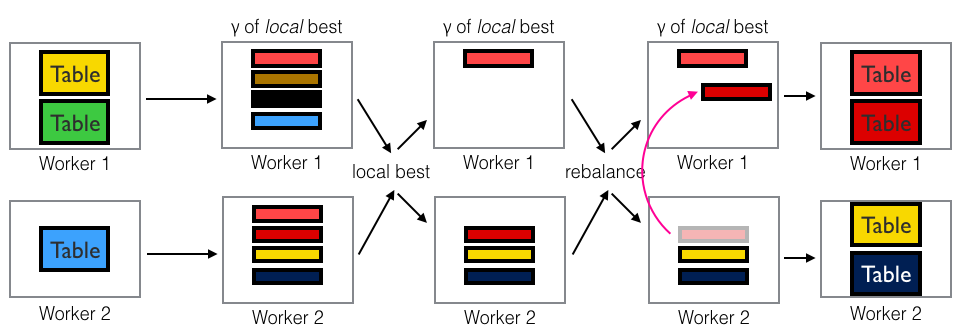
\includegraphics[width=0.6\textwidth]{figures/distributed.png}
    \caption{TODO}
    \label{fig:my_label}
\end{figure*}

\subsection{Parallelism}
The best-first search algorithm also is amenable to parallelization. One can parallelize over the two inner for loops $O \times L$. Each expansion can be forked into its own thread. However, this actually makes the materialization described above a bit more challenging. 

\subsubsection{Shared Memory Parallelization}
The most straight-forward case is when we have access to low-latency shared memory between the expansion threads. In each expansion round, the main thread will assign each expansion node to workers and they will evaluate a given transformation. Each worker will make a copy of $o(R)$ (the node it is expanding) into shared memory. 
If the expanded transformation is within $\gamma$ of the best current result, then it will update the copy, otherwise delete it. The point of synchronization is after all expansions are finished, and the main driver will flush all transformations less than $\gamma$ of the best result, and then assign new workers for the next round. 

\subsubsection{Distributed Parallelization}
In cases, where we do not have access to low-latency shared memory, the communication costs of the above algorithm can be impractical. For each expanded node, the entire table has to be communicated to each of the distributed nodes.
We consider a worker-driver model, and assume that the number of workers is $k$.

\vspace{0.25em} \noindent  \textbf{Initialization. } 
Each worker has a copy of the base relation with no transformations.
In the first round of expansion, the driver assigns to each worker $\frac{|L|}{k}$ expansions. 
Each worker executes each of its assigned expansions, and stores the transformations that are within $\gamma$ of the best local result.

\vspace{0.25em} \noindent  \textbf{Reconciliation. }  Note that the global top-$\gamma$ set is a subset of the union of the all local results.
The workers then communicate the quality of their best transformation. This can be used to reconcile the local materializations to only the global top-$\gamma$ set.
This set is not necessarily balanced, e.g., one worker might have almost all of the top transformations.
The next step is a balancing step, where each worker communicates the number of materialized expansions it currently stores.
The workers with more than $\frac{|O|}{k}$ materialized expansions  randomly select ones to evict, and the driver re-distributes these to nodes with too few materialized expansions.
This is done by communicated the transformation and the result is re-computed on the new worker.
If $|O| < k$, then expansions are chosen at random to be replicated.
The result of the reconciliation step is that all workers have an evenly distributed set of materialized expansions.

\vspace{0.25em} \noindent  \textbf{Next Round. } After reconciliation, each worker is associated with a particular $o \in O$ (or a set of them). To parallelize, the driver must simply ensure that it assigns new expansions only to those workers that have materialized the parent.
The algorithm then repeats, expanding each node locally, and then reconciles the results.




